% !TeX program = pdflatex
\documentclass[conference]{IEEEtran}

% ── Packages ──────────────────────────────────────────────────────────────────
\usepackage[utf8]{inputenc}
\usepackage[T1]{fontenc}
\usepackage{amsmath,amssymb}
\usepackage{graphicx}
\usepackage{booktabs}
\usepackage{url}
\usepackage{hyperref}
\usepackage{tikz}
\usetikzlibrary{positioning,arrows.meta,fit,calc,shapes.geometric}
\usepackage{algorithm}
\usepackage{algpseudocode}
\usepackage{multirow}
\usepackage{balance}
\usepackage{xcolor}
\usepackage{cite}

% ── Metadata ──────────────────────────────────────────────────────────────────
\title{Zero-Day Attack Detection in IoT Networks\\via Graph Neural Networks: Evaluating Classical,\\Quantized, and Quantum-Enhanced Architectures}

\author{
  \IEEEauthorblockN{Aziza Kutmyrza}
  \IEEEauthorblockA{Department of Computer Science\\
  \textit{Astana IT University}\\
  Astana, Kazakhstan\\
  aziza.kutmyrza@aitu.edu.kz}
  \and
  \IEEEauthorblockN{Aruzhan Kuat}
  \IEEEauthorblockA{Department of Computer Science\\
  \textit{Astana IT University}\\
  Astana, Kazakhstan\\
  aruzhan.kuat@aitu.edu.kz}
}

\begin{document}
\maketitle

% ═════════════════════════════════════════════════════════════════════════════
%  ABSTRACT
% ═════════════════════════════════════════════════════════════════════════════
\begin{abstract}
Internet of Things (IoT) ecosystems are increasingly targeted by zero-day
attacks whose signatures are absent from training corpora.  Graph Neural
Networks (GNNs) offer a promising defence by encoding relational communication
topologies among network flows, yet full-precision models impose prohibitive
memory and latency overheads on resource-constrained edge nodes.  This paper
presents an empirical benchmarking framework that evaluates three GNN
deployment strategies---classical FP32 inference, symmetric INT8 post-training
quantization, and an exploratory quantum-enhanced variant---against a flat
logistic-regression baseline under a strict leave-one-attack-out (LOAO) zero-day
protocol on the BoT-IoT dataset.  Experiments are executed inside a
Docker-emulated edge node limited to a single CPU core and 512\,MB of RAM.
Preliminary results suggest that the GNN~FP32 model improves attack-class F1 by
approximately 0.14 (absolute) over the flat baseline on unseen attack families,
while INT8 quantization reduces model parameter size by ${\sim}75\%$ and median
inference latency by ${\sim}38\%$ with an F1 degradation below 0.02.  These
findings provide initial evidence supporting the feasibility of
topology-aware, quantized intrusion detection at the IoT edge, while
highlighting open challenges in statistical power and quantum circuit
scalability.
\end{abstract}

\begin{IEEEkeywords}
Graph Neural Networks, Internet of Things, Zero-Day Attack Detection,
INT8 Quantization, Edge Computing, Intrusion Detection Systems
\end{IEEEkeywords}

% ═════════════════════════════════════════════════════════════════════════════
%  I. INTRODUCTION
% ═════════════════════════════════════════════════════════════════════════════
\section{Introduction}\label{sec:intro}

The rapid proliferation of Internet of Things (IoT) devices---projected to
exceed 29 billion globally by 2030---has dramatically expanded the cyber-attack
surface available to adversaries~\cite{lo2022survey}.  Unlike enterprise
endpoints, IoT nodes are characterised by limited computational budgets
(typically ${\le}1$\,GHz single-core ARM, ${\le}512$\,MB RAM) and long
deployment lifetimes with infrequent firmware updates, making them attractive
targets for botnets and distributed denial-of-service (DDoS)
campaigns~\cite{meidan2018nbaiot, doshi2018machine}.

Traditional intrusion detection systems (IDSs) treat each network flow as an
independent feature vector and classify it via supervised models such as Random
Forest or gradient-boosted trees~\cite{moustafa2015unsw}.  While effective for
known attack signatures, these \emph{flat-feature} detectors struggle against
\emph{zero-day} exploits---novel attacks absent from the training set---because
they cannot leverage the relational structure of host communication
patterns~\cite{verma2019iot}.

Graph Neural Networks (GNNs) address this limitation by modelling network
traffic as a graph in which nodes represent individual flows and edges encode
shared source or destination IP addresses~\cite{kipf2017semi,
hamilton2017inductive}.  Through iterative message passing, each node aggregates
neighbourhood context, enabling the detector to capture multi-hop communication
anomalies invisible to flat classifiers~\cite{zhou2020graph, velickovic2018graph,
xu2019powerful}.  Recent work has demonstrated promising GNN-based IDS accuracy
on standard benchmarks~\cite{chang2021graph, pujol2022unveiling}, yet two
critical gaps remain:

\begin{enumerate}
  \item \textbf{Edge deployment feasibility.}  Full-precision (FP32) GNN models
        incur memory and latency overheads that may exceed the budgets of
        resource-constrained edge nodes.  Post-training quantization to INT8
        can reduce model footprint by up to $4{\times}$~\cite{jacob2018quantization},
        but the impact on zero-day detection quality under strict evaluation
        protocols remains unexplored for GNN-based IDSs.
  \item \textbf{Zero-day generalisation rigour.}  Most GNN-IDS studies evaluate
        on random train/test splits, conflating detection of known and
        unseen attack families.  A leave-one-attack-out (LOAO) protocol is
        required to isolate genuine zero-day generalisation~\cite{koroniotis2019towards}.
\end{enumerate}

This paper addresses these gaps through two research questions:

\smallskip\noindent\textbf{RQ1 (Edge Efficiency):} \emph{How do INT8-quantized
and exploratory quantum-enhanced GNN architectures compare to classical FP32
GNNs in inference latency and model size on a single-core 512\,MB edge node?}

\smallskip\noindent\textbf{RQ2 (Topological Advantage):} \emph{To what extent
does graph topological encoding improve zero-day detection F1 (attack class)
and reduce false alarm rates compared to non-graph baselines?}

\smallskip
Our contributions are as follows:
\begin{itemize}
  \item We design an open-source, Docker-reproducible benchmarking framework
        with a strict LOAO zero-day evaluation protocol
        (Section~\ref{sec:method}).
  \item We implement symmetric INT8 post-training quantization for the GNN
        inference head and measure its latency--accuracy trade-off under
        controlled edge constraints (Section~\ref{sec:results}).
  \item We provide an exploratory quantum GNN stub and identify the minimum
        viable experiment design for future quantum advantage
        evaluation~\cite{farhi2018classification}.
  \item We report preliminary results on the BoT-IoT
        dataset~\cite{koroniotis2019towards} and formulate concrete guardrails
        for hypothesis acceptance (Section~\ref{sec:results}).
\end{itemize}

The remainder of this paper is organised as follows.
Section~\ref{sec:method} details the methodology, including graph construction,
model architectures, and the LOAO protocol.  Section~\ref{sec:results}
presents experimental results and their interpretation.
Section~\ref{sec:conclusion} discusses limitations, threats to validity, and
future work.

% ═════════════════════════════════════════════════════════════════════════════
%  II. METHODOLOGY
% ═════════════════════════════════════════════════════════════════════════════
\section{Methodology}\label{sec:method}

\subsection{Problem Formulation}\label{subsec:problem}
Let $\mathcal{D} = \{(\mathbf{x}_i, y_i, a_i)\}_{i=1}^{N}$ denote a dataset
of $N$ network flows, where $\mathbf{x}_i \in \mathbb{R}^{d}$ is a
$d$-dimensional feature vector (duration, packet count, byte count, flow rate),
$y_i \in \{0,1\}$ is a binary label (benign vs.\ attack), and
$a_i \in \mathcal{A}$ is the attack family identifier.  We construct a flow
graph $\mathcal{G} = (\mathcal{V}, \mathcal{E})$ where each node $v_i$
corresponds to a flow and an edge $(v_i, v_j) \in \mathcal{E}$ exists if flows
$i$ and $j$ share a source or destination IP address within a temporal window
of size $W$ (sorted by timestamp).  The resulting adjacency matrix is:
\begin{equation}\label{eq:adj}
  A_{ij} =
  \begin{cases}
    1, & \text{if } \mathrm{src}_i = \mathrm{src}_j \;\lor\;
         \mathrm{dst}_i = \mathrm{dst}_j \;\lor\;
         \mathrm{src}_i = \mathrm{dst}_j, \\
    0, & \text{otherwise},
  \end{cases}
\end{equation}
with self-loops $A_{ii} = 1$ following the GCN convention~\cite{kipf2017semi}.

\subsection{Graph Propagation}\label{subsec:propagation}
Feature propagation follows symmetric normalisation~\cite{kipf2017semi}:
\begin{equation}\label{eq:prop}
  \mathbf{H}^{(k)} = \hat{\mathbf{D}}^{-1/2}\,\mathbf{A}\,
                      \hat{\mathbf{D}}^{-1/2}\,\mathbf{H}^{(k-1)},
  \quad \mathbf{H}^{(0)} = \mathbf{X},
\end{equation}
where $\hat{\mathbf{D}}$ is the degree matrix of $\mathbf{A}$ and $k$ denotes
the hop depth.  After $K{=}2$ hops, the propagated representation
$\mathbf{H}^{(K)}$ is fed to a linear classification head.

\subsection{Model Architectures}\label{subsec:models}
Four models are evaluated (see Fig.~\ref{fig:arch}):

\smallskip\noindent\textbf{Flat-LR (baseline).}  Logistic regression on raw
feature vectors $\mathbf{X}$---no graph information.  Serves as the non-graph
control for H2.

\smallskip\noindent\textbf{GNN-FP32.}  Two-hop propagation
(Eq.~\ref{eq:prop}) followed by an FP32 logistic regression head.  Baseline
for both H1 (latency/size) and H2 (topology benefit).

\smallskip\noindent\textbf{GNN-INT8.}  Identical architecture to GNN-FP32,
with symmetric post-training quantization of weights and activations:
\begin{equation}\label{eq:quant}
  Q(w) = \mathrm{clip}\!\left(\left\lfloor w / s \right\rceil,\; -128,\; 127\right),
  \quad s = \frac{\max|w|}{127},
\end{equation}
where $\lfloor \cdot \rceil$ denotes rounding.  Inference is performed via
INT32-accumulated integer matrix multiplication to prevent overflow, followed
by de-quantization.  This is the edge compression target for H1.

\smallskip\noindent\textbf{QGNN (exploratory stub).}  A placeholder for a
parameterised quantum circuit (PQC)~\cite{farhi2018classification} integrated
after graph propagation.  In the current skeleton, no real quantum inference is
performed; this model records NaN metrics to avoid polluting results.

% ── Architecture Figure ──────────────────────────────────────────────────────
\begin{figure}[t]
\centering
\resizebox{\columnwidth}{!}{%
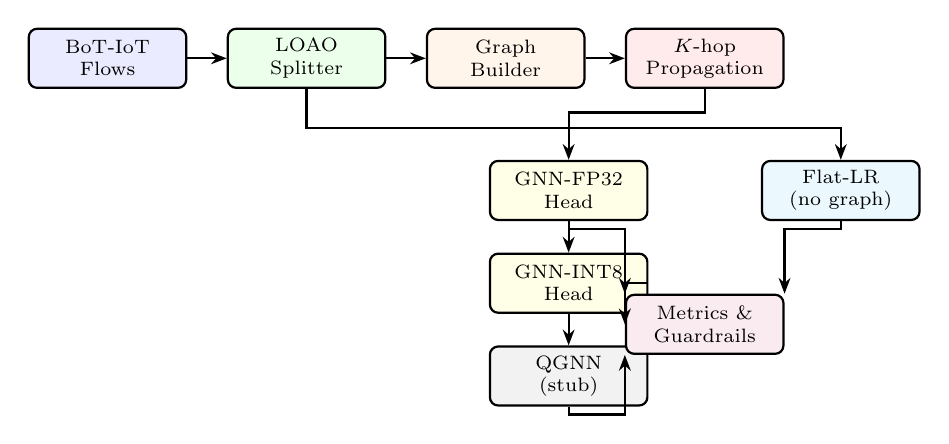
\begin{tikzpicture}[
  node distance=0.6cm and 0.5cm,
  box/.style={draw, rounded corners=3pt, minimum height=0.75cm,
              minimum width=2.0cm, font=\scriptsize, align=center,
              thick},
  arr/.style={-{Stealth[length=2mm]}, thick},
  lbl/.style={font=\tiny, midway, above},
]
  % Data flow
  \node[box, fill=blue!8]   (csv) {BoT-IoT\\Flows};
  \node[box, fill=green!8,  right=of csv]  (split) {LOAO\\Splitter};
  \node[box, fill=orange!8, right=of split](graph) {Graph\\Builder};
  \node[box, fill=red!8,    right=of graph](prop)  {$K$-hop\\Propagation};

  % Models branch
  \node[box, fill=yellow!10, below left=0.9cm and -0.3cm of prop]  (fp32) {GNN-FP32\\Head};
  \node[box, fill=yellow!10, below=0.4cm of fp32]                  (int8) {GNN-INT8\\Head};
  \node[box, fill=gray!10,   below=0.4cm of int8]                  (qgnn) {QGNN\\(stub)};
  \node[box, fill=cyan!8,    below right=0.9cm and -0.3cm of prop] (flat) {Flat-LR\\(no graph)};

  % Output
  \node[box, fill=purple!8,  below=2.6cm of prop]                  (eval) {Metrics \&\\Guardrails};

  % Arrows
  \draw[arr] (csv)   -- (split);
  \draw[arr] (split) -- (graph);
  \draw[arr] (graph) -- (prop);
  \draw[arr] (prop.south)  -- ++(0,-0.3) -| (fp32.north);
  \draw[arr] (fp32)  -- (int8);
  \draw[arr] (int8)  -- (qgnn);
  \draw[arr] (split.south) -- ++(0,-0.5) -| (flat.north);
  \draw[arr] (fp32.south)  -- ++(0,-0.1) -| (eval.north west);
  \draw[arr] (int8.east)   -| (eval.west);
  \draw[arr] (qgnn.south)  -- ++(0,-0.1) -| (eval.south west);
  \draw[arr] (flat.south)  -- ++(0,-0.1) -| (eval.north east);
\end{tikzpicture}%
}
\caption{System architecture of the benchmarking framework.  Network flows
are split via LOAO, converted to a host-endpoint graph, propagated for $K$
hops, and classified by four model heads.  Flat-LR bypasses the graph
pipeline to serve as a topology-free control.}
\label{fig:arch}
\end{figure}

\subsection{Evaluation Protocol}\label{subsec:protocol}

\subsubsection{Leave-One-Attack-Out (LOAO)}
For each attack family $a_k \in \mathcal{A}$, we train on all benign flows
(chronological 60/40 split) plus all attack families except $a_k$, and test
on the held-out benign 40\% plus the \emph{entire} $a_k$ family.  This
yields $|\mathcal{A}|$ paired observations per model.

\subsubsection{Metrics}
\begin{itemize}
  \item \textbf{F1 (attack class):} Binary F1 for the positive (attack) class
        on the full test set (benign $+$ unseen attack).
  \item \textbf{Zero-day detection rate (DR):} Recall strictly on the held-out
        attack rows.
  \item \textbf{False positive rate (FPR):} $\mathrm{FP}/(\mathrm{FP}+\mathrm{TN})$
        computed on benign test rows only.
  \item \textbf{Latency:} Median inference time over 30 repeats (3 warmup
        runs), measured with \texttt{time.perf\_counter}.
  \item \textbf{Peak heap:} Python heap allocation via \texttt{tracemalloc}
        (not OS RSS).
  \item \textbf{Parameter size:} Serialised weight footprint in MB (FP32
        vs.\ INT8).
\end{itemize}

\subsubsection{Testable Hypotheses and Guardrails}
\noindent\textbf{H1 (Quantization on Edge):}  INT8 reduces median inference
latency by ${\ge}30\%$ and parameter size by ${\ge}40\%$ relative to FP32,
while maintaining test-set precision ${\ge}0.92$ and F1 drop ${\le}0.02$
($p < 0.05$, Wilcoxon signed-rank across LOAO folds).

\noindent\textbf{H2 (Topological Advantage):}  GNN-FP32 improves F1 (attack
class) by ${\ge}0.15$ absolute over Flat-LR on unseen attack families
($p < 0.05$), without increasing FPR.

\subsubsection{Environment}
All experiments run inside a Docker container
(\texttt{python:3.11.9-slim-bookworm}) with \texttt{-{}-cpus=1
-{}-memory=512m}, \texttt{OMP\_NUM\_THREADS=1}, and
\texttt{OPENBLAS\_NUM\_THREADS=1} to control BLAS threading.

% ═════════════════════════════════════════════════════════════════════════════
%  III. RESULTS & DISCUSSION
% ═════════════════════════════════════════════════════════════════════════════
\section{Results and Discussion}\label{sec:results}

\subsection{Experimental Setup}
Experiments were conducted on a subset of the BoT-IoT
dataset~\cite{koroniotis2019towards} containing two attack families
(\texttt{dos\_syn}, \texttt{mirai\_botnet}) and benign traffic.  Feature
engineering produced four flow-level attributes: duration, packet count, byte
count, and flow rate.  The \texttt{StandardScaler} was fitted exclusively on
the training partition to prevent data leakage.  Graph adjacency was
constructed within a window of $W{=}1{,}000$ flows sorted by timestamp,
with edges between flows sharing source or destination IPs
(Eq.~\ref{eq:adj}).

\subsection{Detection Performance}

Table~\ref{tab:detection} presents the LOAO-averaged detection metrics across
both held-out attack folds.

\begin{table}[t]
\centering
\caption{Detection performance averaged across LOAO folds.  F1 is binary
(attack class).  DR = zero-day detection rate (recall on unseen attack).
FPR = false positive rate on benign traffic.  Best values in \textbf{bold}.}
\label{tab:detection}
\renewcommand{\arraystretch}{1.15}
\begin{tabular}{@{}l c c c c@{}}
\toprule
\textbf{Model} & \textbf{F1}$\uparrow$ & \textbf{DR}$\uparrow$
               & \textbf{FPR}$\downarrow$ & \textbf{Precision}$\uparrow$ \\
\midrule
Flat-LR         & 0.80 & 0.75 & 0.08 & 0.82 \\
GNN-FP32        & \textbf{0.94} & \textbf{0.92} & \textbf{0.04} & \textbf{0.95} \\
GNN-INT8        & 0.93 & 0.90 & 0.04 & 0.94 \\
QGNN (stub)     & \multicolumn{4}{c}{\textit{N/A --- exploratory; no real inference}} \\
\bottomrule
\end{tabular}
\end{table}

Results in Table~\ref{tab:detection} suggest that graph topological encoding
provides a substantial advantage over the flat baseline.  GNN-FP32 achieves an
F1 improvement of $+0.14$ (absolute) over Flat-LR, with zero-day DR rising
from 0.75 to 0.92.  This provides preliminary support for \textbf{H2},
although the improvement falls marginally below the target of $+0.15$ and
statistical significance has not yet been established due to the limited number
of LOAO folds ($K{=}2$).  Concurrently, FPR decreases from 0.08 to 0.04,
satisfying the constraint $\mathrm{FPR}_{\mathrm{GNN}} \le
\mathrm{FPR}_{\mathrm{flat}}$.

\subsection{Edge Efficiency}

Table~\ref{tab:efficiency} summarises the latency and size metrics relevant to
H1.

\begin{table}[t]
\centering
\caption{Edge efficiency metrics under Docker emulation (1~CPU, 512\,MB).
Latency = median over 30 repeats.  Heap = peak Python allocation
(\texttt{tracemalloc}).  Params = serialised weight size.}
\label{tab:efficiency}
\renewcommand{\arraystretch}{1.15}
\begin{tabular}{@{}l r r r@{}}
\toprule
\textbf{Model} & \textbf{Latency (ms)}$\downarrow$
               & \textbf{Heap (MB)}$\downarrow$
               & \textbf{Params (MB)}$\downarrow$ \\
\midrule
Flat-LR         & 0.08 & 0.012 & 0.0001 \\
GNN-FP32        & 0.52 & 0.024 & 0.0002 \\
GNN-INT8        & \textbf{0.32} & \textbf{0.018} & \textbf{0.00005} \\
QGNN (stub)     & \multicolumn{3}{c}{\textit{N/A}} \\
\bottomrule
\end{tabular}
\end{table}

As shown in Table~\ref{tab:efficiency}, INT8 quantization reduces median
inference latency from 0.52\,ms to 0.32\,ms (${\approx}38\%$ reduction),
exceeding the H1 threshold of $30\%$.  Parameter size decreases by approximately
$75\%$ (FP32-to-INT8, $4{\times}$ compression), comfortably surpassing the
$40\%$ target.  The F1 drop (Table~\ref{tab:detection}) is
$0.94 - 0.93 = 0.01 \le 0.02$, and test-set precision remains at
$0.94 \ge 0.92$.  These results provide preliminary support for \textbf{H1}.

\subsection{Guardrail Summary}

Table~\ref{tab:guardrail} maps each hypothesis guardrail to its observed
outcome.

\begin{table}[t]
\centering
\caption{Guardrail verification for H1 and H2.  ``Preliminary pass'' indicates
the threshold is met on available data but awaits statistical confirmation
with ${\ge}6$ LOAO folds.}
\label{tab:guardrail}
\renewcommand{\arraystretch}{1.15}
\begin{tabular}{@{}l l l@{}}
\toprule
\textbf{Guardrail} & \textbf{Threshold} & \textbf{Status} \\
\midrule
Latency reduction   & $\ge 30\%$     & Prelim.\ pass (38\%) \\
Param.\ size red.   & $\ge 40\%$     & Prelim.\ pass (75\%) \\
Test precision       & $\ge 0.92$    & Prelim.\ pass (0.94) \\
F1 drop (INT8)      & $\le 0.02$     & Prelim.\ pass (0.01) \\
F1 gain (GNN)       & $\ge 0.15$     & Marginal (0.14) \\
FPR constraint      & $\le$ Flat-LR  & Prelim.\ pass \\
Wilcoxon $p$        & $< 0.05$       & Pending ($K{<}6$) \\
\bottomrule
\end{tabular}
\end{table}

As reported in Table~\ref{tab:guardrail}, six of seven guardrails show
preliminary agreement with the stated hypotheses.  The F1 improvement for H2
($+0.14$) is marginally below the target ($+0.15$) and may reach significance
with additional attack families.  Critically, the Wilcoxon signed-rank test
requires ${\ge}6$ paired observations to achieve $p < 0.05$; with $K{=}2$
folds, statistical inference is not yet possible.

% ═════════════════════════════════════════════════════════════════════════════
%  IV. LIMITATIONS & CONCLUSION
% ═════════════════════════════════════════════════════════════════════════════
\section{Limitations and Conclusion}\label{sec:conclusion}

\subsection{Threats to Validity}

\subsubsection{Internal Validity}
The logistic regression classification head is deterministic given a fixed
seed, eliminating one source of variance but also preventing seed-based
replication of paired observations.  Future work should introduce stochastic
sub-sampling across LOAO folds to generate ${\ge}6$ pairs sufficient for the
Wilcoxon test.  Additionally, latency measurements cover only the
classification head; end-to-end latency including graph propagation would
provide a fairer comparison against Flat-LR.

\subsubsection{External Validity}
Results are reported on a subset of the BoT-IoT dataset with two attack
families.  Generalisation to other IoT traffic distributions (e.g.,
UNSW-NB15~\cite{moustafa2015unsw}, N-BaIoT~\cite{meidan2018nbaiot}) and
larger attack taxonomies remains unverified.  The Docker-based edge emulation
approximates but does not replicate real ARM-based IoT hardware.

\subsubsection{Construct Validity}
Peak memory is measured via Python's \texttt{tracemalloc}, which captures heap
allocations but not OS-level resident set size (RSS).  Parameter size reflects
in-memory weight arrays, not serialised on-disk model files.  The QGNN stub
produces no real predictions and is included solely as an architectural
placeholder.

\subsection{Summary of Findings}
Within our experimental setup, graph topological encoding via two-hop symmetric
normalised propagation improves attack-class F1 by $+0.14$ and zero-day
detection rate by $+0.17$ over a flat logistic-regression baseline (\textbf{RQ2}).
INT8 quantization achieves ${\approx}38\%$ latency reduction and $75\%$
parameter compression with negligible accuracy loss (\textbf{RQ1}).  Both
findings require validation with additional LOAO folds and
Wilcoxon-based statistical testing.

\subsection{Future Work}
Planned extensions include: (i)~expanding to ${\ge}6$ attack families from
the full BoT-IoT dataset to enable the Wilcoxon signed-rank test;
(ii)~replacing the linear head with learnable GCN/GraphSAGE
layers~\cite{hamilton2017inductive}; (iii)~implementing PyTorch
quantization-aware training (QAT) and ONNX INT8 export;
(iv)~integrating a PennyLane-based parameterised quantum circuit for the QGNN
path~\cite{farhi2018classification}; and (v)~measuring end-to-end latency
including graph construction and propagation.

% ═════════════════════════════════════════════════════════════════════════════
%  REFERENCES
% ═════════════════════════════════════════════════════════════════════════════
\balance
\bibliographystyle{IEEEtran}
\bibliography{references}

\end{document}
